\documentclass[14pt]{extbook}
\usepackage{multicol, enumerate, enumitem, hyperref, color, soul, setspace, parskip, fancyhdr} %General Packages
\usepackage{amssymb, amsthm, amsmath, latexsym, units, mathtools} %Math Packages
\everymath{\displaystyle} %All math in Display Style
% Packages with additional options
\usepackage[headsep=0.5cm,headheight=12pt, left=1 in,right= 1 in,top= 1 in,bottom= 1 in]{geometry}
\usepackage[usenames,dvipsnames]{xcolor}
\usepackage{dashrule}  % Package to use the command below to create lines between items
\newcommand{\litem}[1]{\item#1\hspace*{-1cm}\rule{\textwidth}{0.4pt}}
\pagestyle{fancy}
\lhead{Progress Quiz 5}
\chead{}
\rhead{Version ALL}
\lfoot{8497-6012}
\cfoot{}
\rfoot{Summer C 2021}
\begin{document}

\begin{enumerate}
\litem{
Construct the lowest-degree polynomial given the zeros below. Then, choose the intervals that contain the coefficients of the polynomial in the form $x^3+bx^2+cx+d$.\[ -5 + 4 i \text{ and } 4 \]\begin{enumerate}[label=\Alph*.]
\item \( b \in [5, 14], c \in [-1, 5], \text{ and } d \in [-165, -162] \)
\item \( b \in [-2, 4], c \in [-1, 5], \text{ and } d \in [-22, -18] \)
\item \( b \in [-2, 4], c \in [-10, -7], \text{ and } d \in [11, 20] \)
\item \( b \in [-12, -3], c \in [-1, 5], \text{ and } d \in [164, 169] \)
\item \( \text{None of the above.} \)

\end{enumerate} }
\litem{
Construct the lowest-degree polynomial given the zeros below. Then, choose the intervals that contain the coefficients of the polynomial in the form $ax^3+bx^2+cx+d$.\[ \frac{7}{4}, 5, \text{ and } \frac{7}{3} \]\begin{enumerate}[label=\Alph*.]
\item \( a \in [12, 14], b \in [-112, -107], c \in [293, 297], \text{ and } d \in [245, 252] \)
\item \( a \in [12, 14], b \in [-76, -65], c \in [-15, -8], \text{ and } d \in [245, 252] \)
\item \( a \in [12, 14], b \in [108, 115], c \in [293, 297], \text{ and } d \in [245, 252] \)
\item \( a \in [12, 14], b \in [-112, -107], c \in [293, 297], \text{ and } d \in [-246, -240] \)
\item \( a \in [12, 14], b \in [49, 58], c \in [-88, -83], \text{ and } d \in [-246, -240] \)

\end{enumerate} }
\litem{
Describe the end behavior of the polynomial below.\[ f(x) = -5(x + 3)^{4}(x - 3)^{5}(x + 2)^{3}(x - 2)^{5} \]\begin{enumerate}[label=\Alph*.]
\begin{multicols}{2}\item 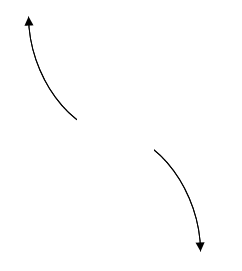
\includegraphics[width = 0.3\textwidth]{../Figures/polyEndBehaviorAA.png}\item 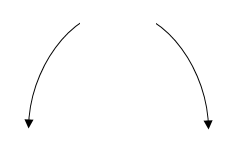
\includegraphics[width = 0.3\textwidth]{../Figures/polyEndBehaviorBA.png}\item 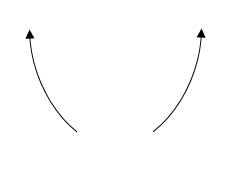
\includegraphics[width = 0.3\textwidth]{../Figures/polyEndBehaviorCA.png}\item 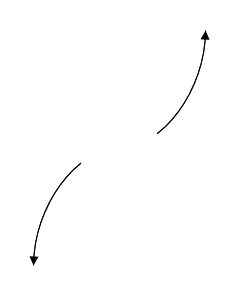
\includegraphics[width = 0.3\textwidth]{../Figures/polyEndBehaviorDA.png}\end{multicols}\item None of the above.
\end{enumerate} }
\litem{
Which of the following equations \textit{could} be of the graph presented below?
\begin{center}
    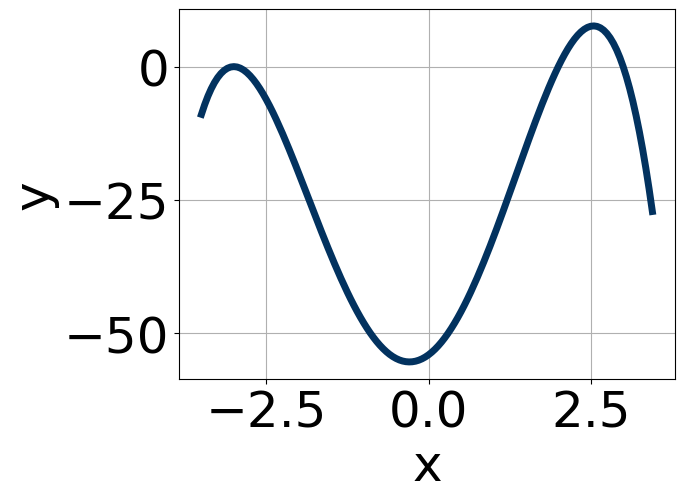
\includegraphics[width=0.5\textwidth]{../Figures/polyGraphToFunctionCopyA.png}
\end{center}
\begin{enumerate}[label=\Alph*.]
\item \( 18(x + 3)^{10} (x - 3)^{9} (x - 2)^{7} \)
\item \( -5(x + 3)^{6} (x - 3)^{5} (x - 2)^{9} \)
\item \( 4(x + 3)^{4} (x - 3)^{9} (x - 2)^{4} \)
\item \( -16(x + 3)^{5} (x - 3)^{8} (x - 2)^{7} \)
\item \( -13(x + 3)^{10} (x - 3)^{8} (x - 2)^{11} \)

\end{enumerate} }
\litem{
Construct the lowest-degree polynomial given the zeros below. Then, choose the intervals that contain the coefficients of the polynomial in the form $ax^3+bx^2+cx+d$.\[ \frac{-1}{2}, \frac{5}{4}, \text{ and } \frac{7}{5} \]\begin{enumerate}[label=\Alph*.]
\item \( a \in [35, 45], b \in [-86, -81], c \in [16, 18], \text{ and } d \in [32, 42] \)
\item \( a \in [35, 45], b \in [-128, -124], c \in [121, 126], \text{ and } d \in [-38, -33] \)
\item \( a \in [35, 45], b \in [-33, -17], c \in [-75, -64], \text{ and } d \in [32, 42] \)
\item \( a \in [35, 45], b \in [-86, -81], c \in [16, 18], \text{ and } d \in [-38, -33] \)
\item \( a \in [35, 45], b \in [81, 94], c \in [16, 18], \text{ and } d \in [-38, -33] \)

\end{enumerate} }
\litem{
Which of the following equations \textit{could} be of the graph presented below?
\begin{center}
    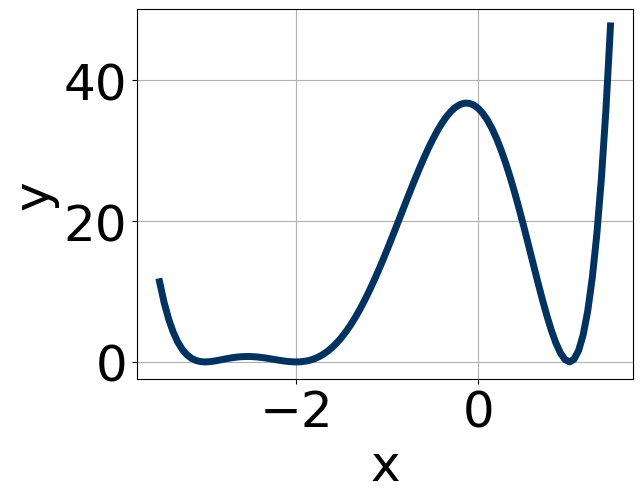
\includegraphics[width=0.5\textwidth]{../Figures/polyGraphToFunctionA.png}
\end{center}
\begin{enumerate}[label=\Alph*.]
\item \( 8(x + 2)^{8} (x + 3)^{6} (x - 1)^{6} \)
\item \( -12(x + 2)^{4} (x + 3)^{8} (x - 1)^{10} \)
\item \( 10(x + 2)^{6} (x + 3)^{6} (x - 1)^{5} \)
\item \( -13(x + 2)^{10} (x + 3)^{8} (x - 1)^{9} \)
\item \( 19(x + 2)^{10} (x + 3)^{11} (x - 1)^{9} \)

\end{enumerate} }
\litem{
Describe the zero behavior of the zero $x = 3$ of the polynomial below.\[ f(x) = -2(x - 2)^{6}(x + 2)^{3}(x + 3)^{11}(x - 3)^{6} \]\begin{enumerate}[label=\Alph*.]
\begin{multicols}{2}\item 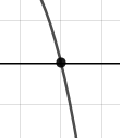
\includegraphics[width = 0.3\textwidth]{../Figures/polyZeroBehaviorAA.png}\item 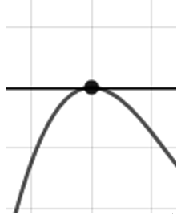
\includegraphics[width = 0.3\textwidth]{../Figures/polyZeroBehaviorBA.png}\item 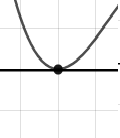
\includegraphics[width = 0.3\textwidth]{../Figures/polyZeroBehaviorCA.png}\item 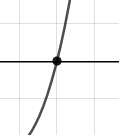
\includegraphics[width = 0.3\textwidth]{../Figures/polyZeroBehaviorDA.png}\end{multicols}\item None of the above.
\end{enumerate} }
\litem{
Describe the zero behavior of the zero $x = 2$ of the polynomial below.\[ f(x) = -2(x - 2)^{2}(x + 2)^{7}(x + 9)^{4}(x - 9)^{8} \]\begin{enumerate}[label=\Alph*.]
\begin{multicols}{2}\item 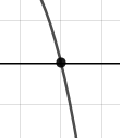
\includegraphics[width = 0.3\textwidth]{../Figures/polyZeroBehaviorCopyAA.png}\item 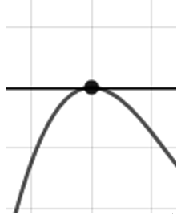
\includegraphics[width = 0.3\textwidth]{../Figures/polyZeroBehaviorCopyBA.png}\item 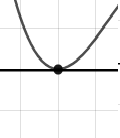
\includegraphics[width = 0.3\textwidth]{../Figures/polyZeroBehaviorCopyCA.png}\item 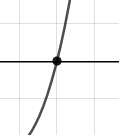
\includegraphics[width = 0.3\textwidth]{../Figures/polyZeroBehaviorCopyDA.png}\end{multicols}\item None of the above.
\end{enumerate} }
\litem{
Construct the lowest-degree polynomial given the zeros below. Then, choose the intervals that contain the coefficients of the polynomial in the form $x^3+bx^2+cx+d$.\[ -2 + 2 i \text{ and } 1 \]\begin{enumerate}[label=\Alph*.]
\item \( b \in [-3.8, -1.5], c \in [2.1, 5.2], \text{ and } d \in [6.4, 9.3] \)
\item \( b \in [0.7, 2.7], c \in [-3.6, -0.8], \text{ and } d \in [0.3, 4.3] \)
\item \( b \in [2, 4.5], c \in [2.1, 5.2], \text{ and } d \in [-8.4, -7.4] \)
\item \( b \in [0.7, 2.7], c \in [-0.3, 2.5], \text{ and } d \in [-4.2, -1.1] \)
\item \( \text{None of the above.} \)

\end{enumerate} }
\litem{
Describe the end behavior of the polynomial below.\[ f(x) = 6(x + 3)^{3}(x - 3)^{6}(x - 2)^{5}(x + 2)^{6} \]\begin{enumerate}[label=\Alph*.]
\begin{multicols}{2}\item 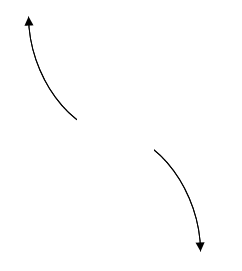
\includegraphics[width = 0.3\textwidth]{../Figures/polyEndBehaviorCopyAA.png}\item 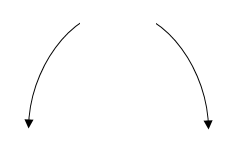
\includegraphics[width = 0.3\textwidth]{../Figures/polyEndBehaviorCopyBA.png}\item 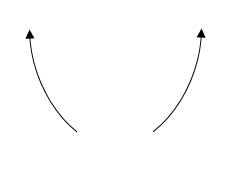
\includegraphics[width = 0.3\textwidth]{../Figures/polyEndBehaviorCopyCA.png}\item 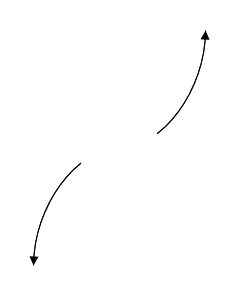
\includegraphics[width = 0.3\textwidth]{../Figures/polyEndBehaviorCopyDA.png}\end{multicols}\item None of the above.
\end{enumerate} }
\litem{
Construct the lowest-degree polynomial given the zeros below. Then, choose the intervals that contain the coefficients of the polynomial in the form $x^3+bx^2+cx+d$.\[ -5 + 4 i \text{ and } 1 \]\begin{enumerate}[label=\Alph*.]
\item \( b \in [7, 12], c \in [31, 38], \text{ and } d \in [-48, -38] \)
\item \( b \in [0, 5], c \in [-2, 10], \text{ and } d \in [-10, -2] \)
\item \( b \in [-10, -7], c \in [31, 38], \text{ and } d \in [35, 42] \)
\item \( b \in [0, 5], c \in [-7, 0], \text{ and } d \in [2, 5] \)
\item \( \text{None of the above.} \)

\end{enumerate} }
\litem{
Construct the lowest-degree polynomial given the zeros below. Then, choose the intervals that contain the coefficients of the polynomial in the form $ax^3+bx^2+cx+d$.\[ \frac{-7}{3}, \frac{-3}{2}, \text{ and } -1 \]\begin{enumerate}[label=\Alph*.]
\item \( a \in [0, 8], b \in [-18, -13], c \in [-7, -1], \text{ and } d \in [20, 27] \)
\item \( a \in [0, 8], b \in [-31, -26], c \in [43, 48], \text{ and } d \in [-21, -18] \)
\item \( a \in [0, 8], b \in [-2, 12], c \in [-29, -22], \text{ and } d \in [-21, -18] \)
\item \( a \in [0, 8], b \in [26, 34], c \in [43, 48], \text{ and } d \in [-21, -18] \)
\item \( a \in [0, 8], b \in [26, 34], c \in [43, 48], \text{ and } d \in [20, 27] \)

\end{enumerate} }
\litem{
Describe the end behavior of the polynomial below.\[ f(x) = 8(x + 3)^{5}(x - 3)^{10}(x + 9)^{2}(x - 9)^{3} \]\begin{enumerate}[label=\Alph*.]
\begin{multicols}{2}\item 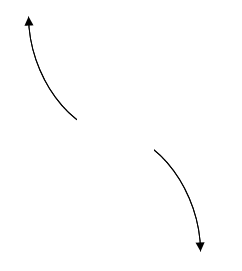
\includegraphics[width = 0.3\textwidth]{../Figures/polyEndBehaviorAB.png}\item 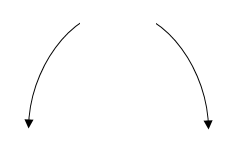
\includegraphics[width = 0.3\textwidth]{../Figures/polyEndBehaviorBB.png}\item 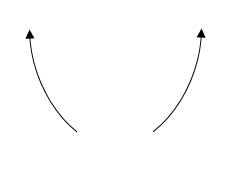
\includegraphics[width = 0.3\textwidth]{../Figures/polyEndBehaviorCB.png}\item 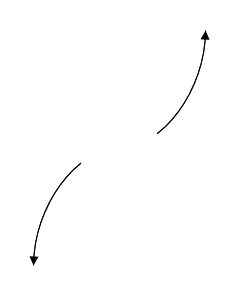
\includegraphics[width = 0.3\textwidth]{../Figures/polyEndBehaviorDB.png}\end{multicols}\item None of the above.
\end{enumerate} }
\litem{
Which of the following equations \textit{could} be of the graph presented below?
\begin{center}
    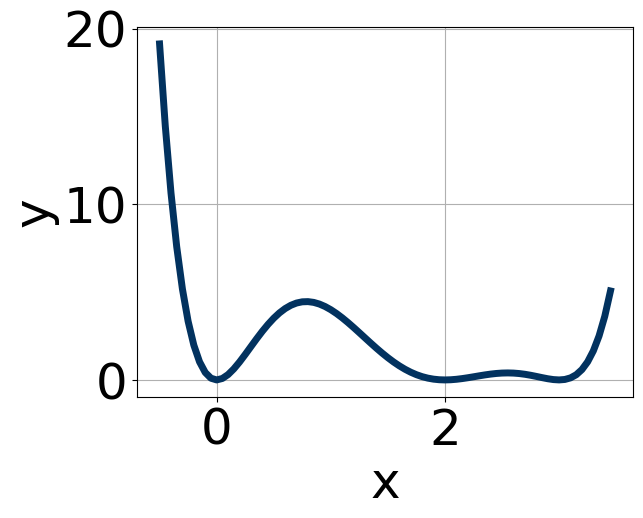
\includegraphics[width=0.5\textwidth]{../Figures/polyGraphToFunctionCopyB.png}
\end{center}
\begin{enumerate}[label=\Alph*.]
\item \( -6x^{10} (x - 3)^{8} (x - 2)^{11} \)
\item \( -12x^{8} (x - 3)^{10} (x - 2)^{10} \)
\item \( 20x^{8} (x - 3)^{4} (x - 2)^{6} \)
\item \( 19x^{10} (x - 3)^{10} (x - 2)^{5} \)
\item \( 17x^{7} (x - 3)^{8} (x - 2)^{7} \)

\end{enumerate} }
\litem{
Construct the lowest-degree polynomial given the zeros below. Then, choose the intervals that contain the coefficients of the polynomial in the form $ax^3+bx^2+cx+d$.\[ \frac{-3}{4}, 4, \text{ and } \frac{4}{3} \]\begin{enumerate}[label=\Alph*.]
\item \( a \in [6, 19], b \in [54, 56], c \in [13, 20], \text{ and } d \in [-52, -44] \)
\item \( a \in [6, 19], b \in [-58, -53], c \in [13, 20], \text{ and } d \in [-52, -44] \)
\item \( a \in [6, 19], b \in [-58, -53], c \in [13, 20], \text{ and } d \in [47, 52] \)
\item \( a \in [6, 19], b \in [22, 29], c \in [-90, -84], \text{ and } d \in [47, 52] \)
\item \( a \in [6, 19], b \in [-77, -65], c \in [111, 121], \text{ and } d \in [-52, -44] \)

\end{enumerate} }
\litem{
Which of the following equations \textit{could} be of the graph presented below?
\begin{center}
    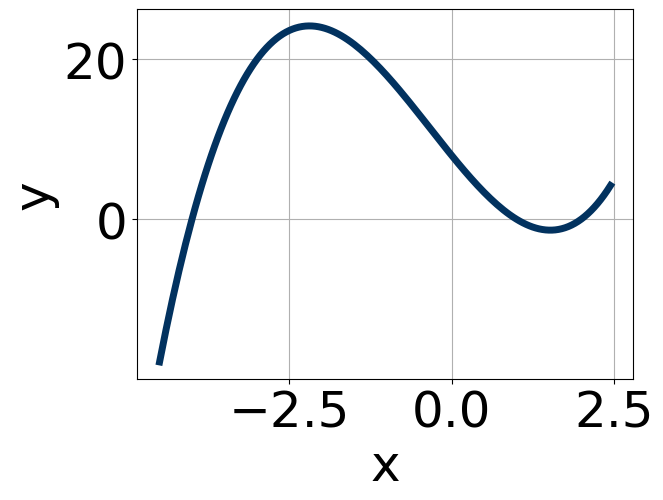
\includegraphics[width=0.5\textwidth]{../Figures/polyGraphToFunctionB.png}
\end{center}
\begin{enumerate}[label=\Alph*.]
\item \( -7(x - 1)^{8} (x - 2)^{7} (x + 4)^{11} \)
\item \( -17(x - 1)^{5} (x - 2)^{9} (x + 4)^{9} \)
\item \( 11(x - 1)^{7} (x - 2)^{9} (x + 4)^{7} \)
\item \( 20(x - 1)^{10} (x - 2)^{8} (x + 4)^{11} \)
\item \( 18(x - 1)^{6} (x - 2)^{11} (x + 4)^{5} \)

\end{enumerate} }
\litem{
Describe the zero behavior of the zero $x = -4$ of the polynomial below.\[ f(x) = 4(x + 4)^{8}(x - 4)^{13}(x - 8)^{2}(x + 8)^{6} \]\begin{enumerate}[label=\Alph*.]
\begin{multicols}{2}\item 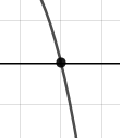
\includegraphics[width = 0.3\textwidth]{../Figures/polyZeroBehaviorAB.png}\item 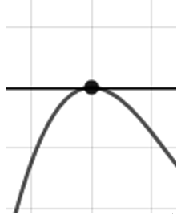
\includegraphics[width = 0.3\textwidth]{../Figures/polyZeroBehaviorBB.png}\item 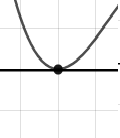
\includegraphics[width = 0.3\textwidth]{../Figures/polyZeroBehaviorCB.png}\item 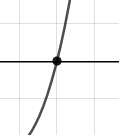
\includegraphics[width = 0.3\textwidth]{../Figures/polyZeroBehaviorDB.png}\end{multicols}\item None of the above.
\end{enumerate} }
\litem{
Describe the zero behavior of the zero $x = -6$ of the polynomial below.\[ f(x) = -4(x - 8)^{12}(x + 8)^{8}(x + 6)^{11}(x - 6)^{8} \]\begin{enumerate}[label=\Alph*.]
\begin{multicols}{2}\item 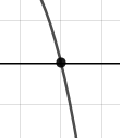
\includegraphics[width = 0.3\textwidth]{../Figures/polyZeroBehaviorCopyAB.png}\item 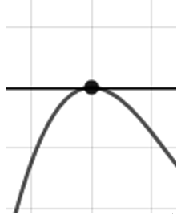
\includegraphics[width = 0.3\textwidth]{../Figures/polyZeroBehaviorCopyBB.png}\item 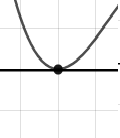
\includegraphics[width = 0.3\textwidth]{../Figures/polyZeroBehaviorCopyCB.png}\item 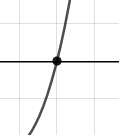
\includegraphics[width = 0.3\textwidth]{../Figures/polyZeroBehaviorCopyDB.png}\end{multicols}\item None of the above.
\end{enumerate} }
\litem{
Construct the lowest-degree polynomial given the zeros below. Then, choose the intervals that contain the coefficients of the polynomial in the form $x^3+bx^2+cx+d$.\[ -5 + 4 i \text{ and } 4 \]\begin{enumerate}[label=\Alph*.]
\item \( b \in [-7.2, -3.1], c \in [-6, 9], \text{ and } d \in [157, 173] \)
\item \( b \in [-1.8, 4.3], c \in [-6, 9], \text{ and } d \in [-26, -16] \)
\item \( b \in [-1.8, 4.3], c \in [-10, -5], \text{ and } d \in [16, 23] \)
\item \( b \in [5.4, 7.5], c \in [-6, 9], \text{ and } d \in [-165, -163] \)
\item \( \text{None of the above.} \)

\end{enumerate} }
\litem{
Describe the end behavior of the polynomial below.\[ f(x) = 4(x - 9)^{3}(x + 9)^{8}(x - 8)^{4}(x + 8)^{4} \]\begin{enumerate}[label=\Alph*.]
\begin{multicols}{2}\item 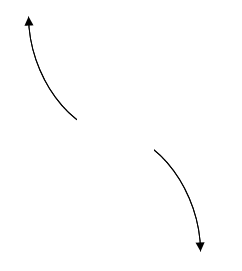
\includegraphics[width = 0.3\textwidth]{../Figures/polyEndBehaviorCopyAB.png}\item 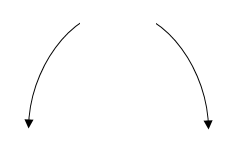
\includegraphics[width = 0.3\textwidth]{../Figures/polyEndBehaviorCopyBB.png}\item 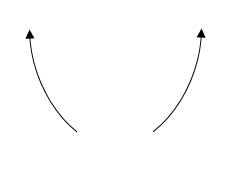
\includegraphics[width = 0.3\textwidth]{../Figures/polyEndBehaviorCopyCB.png}\item 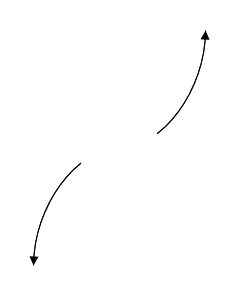
\includegraphics[width = 0.3\textwidth]{../Figures/polyEndBehaviorCopyDB.png}\end{multicols}\item None of the above.
\end{enumerate} }
\litem{
Construct the lowest-degree polynomial given the zeros below. Then, choose the intervals that contain the coefficients of the polynomial in the form $x^3+bx^2+cx+d$.\[ 4 - 2 i \text{ and } -4 \]\begin{enumerate}[label=\Alph*.]
\item \( b \in [2.8, 5.1], c \in [-12, -11], \text{ and } d \in [-87, -78] \)
\item \( b \in [-7.8, -3.5], c \in [-12, -11], \text{ and } d \in [78, 84] \)
\item \( b \in [-0.6, 1.1], c \in [3, 7], \text{ and } d \in [3, 9] \)
\item \( b \in [-0.6, 1.1], c \in [0, 5], \text{ and } d \in [-20, -13] \)
\item \( \text{None of the above.} \)

\end{enumerate} }
\litem{
Construct the lowest-degree polynomial given the zeros below. Then, choose the intervals that contain the coefficients of the polynomial in the form $ax^3+bx^2+cx+d$.\[ -6, \frac{1}{3}, \text{ and } \frac{-3}{2} \]\begin{enumerate}[label=\Alph*.]
\item \( a \in [6, 12], b \in [-25.3, -24.5], c \in [-64, -61], \text{ and } d \in [-24, -15] \)
\item \( a \in [6, 12], b \in [40.1, 45.7], c \in [33, 40], \text{ and } d \in [-24, -15] \)
\item \( a \in [6, 12], b \in [-30.7, -26], c \in [-53, -38], \text{ and } d \in [11, 26] \)
\item \( a \in [6, 12], b \in [-44.1, -41], c \in [33, 40], \text{ and } d \in [11, 26] \)
\item \( a \in [6, 12], b \in [40.1, 45.7], c \in [33, 40], \text{ and } d \in [11, 26] \)

\end{enumerate} }
\litem{
Describe the end behavior of the polynomial below.\[ f(x) = -6(x + 7)^{5}(x - 7)^{10}(x - 8)^{3}(x + 8)^{3} \]\begin{enumerate}[label=\Alph*.]
\begin{multicols}{2}\item 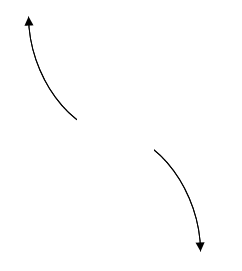
\includegraphics[width = 0.3\textwidth]{../Figures/polyEndBehaviorAC.png}\item 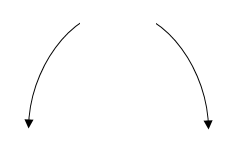
\includegraphics[width = 0.3\textwidth]{../Figures/polyEndBehaviorBC.png}\item 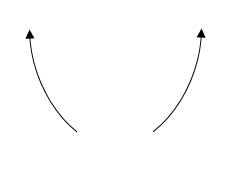
\includegraphics[width = 0.3\textwidth]{../Figures/polyEndBehaviorCC.png}\item 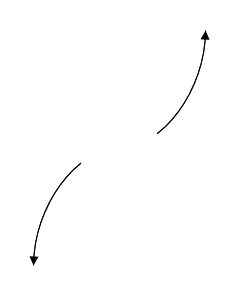
\includegraphics[width = 0.3\textwidth]{../Figures/polyEndBehaviorDC.png}\end{multicols}\item None of the above.
\end{enumerate} }
\litem{
Which of the following equations \textit{could} be of the graph presented below?
\begin{center}
    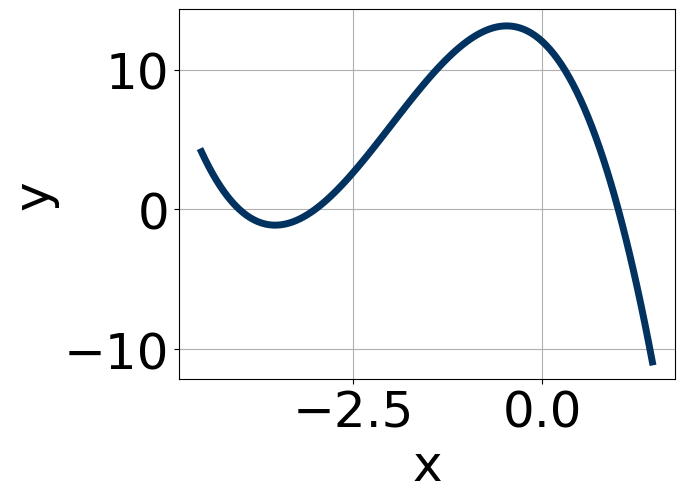
\includegraphics[width=0.5\textwidth]{../Figures/polyGraphToFunctionCopyC.png}
\end{center}
\begin{enumerate}[label=\Alph*.]
\item \( -10(x + 3)^{10} (x - 1)^{11} (x + 4)^{9} \)
\item \( 9(x + 3)^{10} (x - 1)^{5} (x + 4)^{5} \)
\item \( 16(x + 3)^{7} (x - 1)^{7} (x + 4)^{5} \)
\item \( -17(x + 3)^{10} (x - 1)^{6} (x + 4)^{11} \)
\item \( -13(x + 3)^{9} (x - 1)^{7} (x + 4)^{5} \)

\end{enumerate} }
\litem{
Construct the lowest-degree polynomial given the zeros below. Then, choose the intervals that contain the coefficients of the polynomial in the form $ax^3+bx^2+cx+d$.\[ \frac{1}{4}, \frac{7}{4}, \text{ and } \frac{-2}{3} \]\begin{enumerate}[label=\Alph*.]
\item \( a \in [45, 50], b \in [123, 130], c \in [83, 89], \text{ and } d \in [12, 19] \)
\item \( a \in [45, 50], b \in [-41, -33], c \in [-70, -66], \text{ and } d \in [-20, -13] \)
\item \( a \in [45, 50], b \in [-66, -60], c \in [-43, -33], \text{ and } d \in [12, 19] \)
\item \( a \in [45, 50], b \in [-66, -60], c \in [-43, -33], \text{ and } d \in [-20, -13] \)
\item \( a \in [45, 50], b \in [64, 70], c \in [-43, -33], \text{ and } d \in [-20, -13] \)

\end{enumerate} }
\litem{
Which of the following equations \textit{could} be of the graph presented below?
\begin{center}
    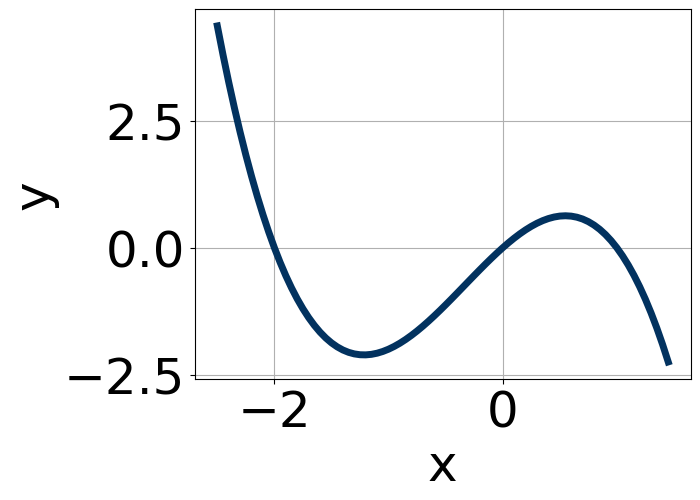
\includegraphics[width=0.5\textwidth]{../Figures/polyGraphToFunctionC.png}
\end{center}
\begin{enumerate}[label=\Alph*.]
\item \( 11x^{9} (x + 2)^{6} (x - 1)^{5} \)
\item \( 11x^{11} (x + 2)^{5} (x - 1)^{5} \)
\item \( -12x^{5} (x + 2)^{5} (x - 1)^{9} \)
\item \( -6x^{7} (x + 2)^{10} (x - 1)^{7} \)
\item \( -9x^{6} (x + 2)^{4} (x - 1)^{7} \)

\end{enumerate} }
\litem{
Describe the zero behavior of the zero $x = -8$ of the polynomial below.\[ f(x) = 3(x + 2)^{5}(x - 2)^{2}(x + 8)^{7}(x - 8)^{2} \]\begin{enumerate}[label=\Alph*.]
\begin{multicols}{2}\item 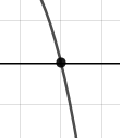
\includegraphics[width = 0.3\textwidth]{../Figures/polyZeroBehaviorAC.png}\item 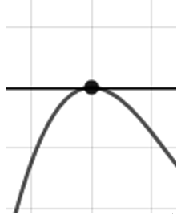
\includegraphics[width = 0.3\textwidth]{../Figures/polyZeroBehaviorBC.png}\item 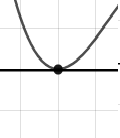
\includegraphics[width = 0.3\textwidth]{../Figures/polyZeroBehaviorCC.png}\item 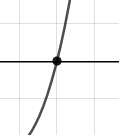
\includegraphics[width = 0.3\textwidth]{../Figures/polyZeroBehaviorDC.png}\end{multicols}\item None of the above.
\end{enumerate} }
\litem{
Describe the zero behavior of the zero $x = -5$ of the polynomial below.\[ f(x) = 7(x - 5)^{2}(x + 5)^{5}(x + 9)^{8}(x - 9)^{11} \]\begin{enumerate}[label=\Alph*.]
\begin{multicols}{2}\item 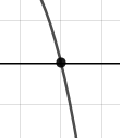
\includegraphics[width = 0.3\textwidth]{../Figures/polyZeroBehaviorCopyAC.png}\item 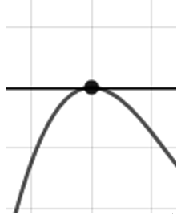
\includegraphics[width = 0.3\textwidth]{../Figures/polyZeroBehaviorCopyBC.png}\item 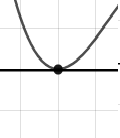
\includegraphics[width = 0.3\textwidth]{../Figures/polyZeroBehaviorCopyCC.png}\item 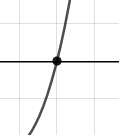
\includegraphics[width = 0.3\textwidth]{../Figures/polyZeroBehaviorCopyDC.png}\end{multicols}\item None of the above.
\end{enumerate} }
\litem{
Construct the lowest-degree polynomial given the zeros below. Then, choose the intervals that contain the coefficients of the polynomial in the form $x^3+bx^2+cx+d$.\[ -4 + 3 i \text{ and } 3 \]\begin{enumerate}[label=\Alph*.]
\item \( b \in [-0.5, 2], c \in [-15, -4], \text{ and } d \in [7, 12] \)
\item \( b \in [3.6, 8.1], c \in [0, 5], \text{ and } d \in [-77, -74] \)
\item \( b \in [-5.2, 0.5], c \in [0, 5], \text{ and } d \in [70, 77] \)
\item \( b \in [-0.5, 2], c \in [0, 5], \text{ and } d \in [-14, -5] \)
\item \( \text{None of the above.} \)

\end{enumerate} }
\litem{
Describe the end behavior of the polynomial below.\[ f(x) = 5(x - 6)^{2}(x + 6)^{3}(x + 3)^{5}(x - 3)^{7} \]\begin{enumerate}[label=\Alph*.]
\begin{multicols}{2}\item \includegraphics[width = 0.3\textwidth]{../Figures/polyEndBehaviorCopyAC.png}\item \includegraphics[width = 0.3\textwidth]{../Figures/polyEndBehaviorCopyBC.png}\item \includegraphics[width = 0.3\textwidth]{../Figures/polyEndBehaviorCopyCC.png}\item \includegraphics[width = 0.3\textwidth]{../Figures/polyEndBehaviorCopyDC.png}\end{multicols}\item None of the above.
\end{enumerate} }
\end{enumerate}

\end{document}